\documentclass[]{article}
\usepackage{lmodern}
\usepackage{amssymb,amsmath}
\usepackage{ifxetex,ifluatex}
\usepackage{fixltx2e} % provides \textsubscript
\ifnum 0\ifxetex 1\fi\ifluatex 1\fi=0 % if pdftex
  \usepackage[T1]{fontenc}
  \usepackage[utf8]{inputenc}
\else % if luatex or xelatex
  \ifxetex
    \usepackage{mathspec}
  \else
    \usepackage{fontspec}
  \fi
  \defaultfontfeatures{Ligatures=TeX,Scale=MatchLowercase}
\fi
% use upquote if available, for straight quotes in verbatim environments
\IfFileExists{upquote.sty}{\usepackage{upquote}}{}
% use microtype if available
\IfFileExists{microtype.sty}{%
\usepackage{microtype}
\UseMicrotypeSet[protrusion]{basicmath} % disable protrusion for tt fonts
}{}
\usepackage[margin=1in]{geometry}
\usepackage{hyperref}
\hypersetup{unicode=true,
            pdfborder={0 0 0},
            breaklinks=true}
\urlstyle{same}  % don't use monospace font for urls
\usepackage{color}
\usepackage{fancyvrb}
\newcommand{\VerbBar}{|}
\newcommand{\VERB}{\Verb[commandchars=\\\{\}]}
\DefineVerbatimEnvironment{Highlighting}{Verbatim}{commandchars=\\\{\}}
% Add ',fontsize=\small' for more characters per line
\usepackage{framed}
\definecolor{shadecolor}{RGB}{248,248,248}
\newenvironment{Shaded}{\begin{snugshade}}{\end{snugshade}}
\newcommand{\AlertTok}[1]{\textcolor[rgb]{0.94,0.16,0.16}{#1}}
\newcommand{\AnnotationTok}[1]{\textcolor[rgb]{0.56,0.35,0.01}{\textbf{\textit{#1}}}}
\newcommand{\AttributeTok}[1]{\textcolor[rgb]{0.77,0.63,0.00}{#1}}
\newcommand{\BaseNTok}[1]{\textcolor[rgb]{0.00,0.00,0.81}{#1}}
\newcommand{\BuiltInTok}[1]{#1}
\newcommand{\CharTok}[1]{\textcolor[rgb]{0.31,0.60,0.02}{#1}}
\newcommand{\CommentTok}[1]{\textcolor[rgb]{0.56,0.35,0.01}{\textit{#1}}}
\newcommand{\CommentVarTok}[1]{\textcolor[rgb]{0.56,0.35,0.01}{\textbf{\textit{#1}}}}
\newcommand{\ConstantTok}[1]{\textcolor[rgb]{0.00,0.00,0.00}{#1}}
\newcommand{\ControlFlowTok}[1]{\textcolor[rgb]{0.13,0.29,0.53}{\textbf{#1}}}
\newcommand{\DataTypeTok}[1]{\textcolor[rgb]{0.13,0.29,0.53}{#1}}
\newcommand{\DecValTok}[1]{\textcolor[rgb]{0.00,0.00,0.81}{#1}}
\newcommand{\DocumentationTok}[1]{\textcolor[rgb]{0.56,0.35,0.01}{\textbf{\textit{#1}}}}
\newcommand{\ErrorTok}[1]{\textcolor[rgb]{0.64,0.00,0.00}{\textbf{#1}}}
\newcommand{\ExtensionTok}[1]{#1}
\newcommand{\FloatTok}[1]{\textcolor[rgb]{0.00,0.00,0.81}{#1}}
\newcommand{\FunctionTok}[1]{\textcolor[rgb]{0.00,0.00,0.00}{#1}}
\newcommand{\ImportTok}[1]{#1}
\newcommand{\InformationTok}[1]{\textcolor[rgb]{0.56,0.35,0.01}{\textbf{\textit{#1}}}}
\newcommand{\KeywordTok}[1]{\textcolor[rgb]{0.13,0.29,0.53}{\textbf{#1}}}
\newcommand{\NormalTok}[1]{#1}
\newcommand{\OperatorTok}[1]{\textcolor[rgb]{0.81,0.36,0.00}{\textbf{#1}}}
\newcommand{\OtherTok}[1]{\textcolor[rgb]{0.56,0.35,0.01}{#1}}
\newcommand{\PreprocessorTok}[1]{\textcolor[rgb]{0.56,0.35,0.01}{\textit{#1}}}
\newcommand{\RegionMarkerTok}[1]{#1}
\newcommand{\SpecialCharTok}[1]{\textcolor[rgb]{0.00,0.00,0.00}{#1}}
\newcommand{\SpecialStringTok}[1]{\textcolor[rgb]{0.31,0.60,0.02}{#1}}
\newcommand{\StringTok}[1]{\textcolor[rgb]{0.31,0.60,0.02}{#1}}
\newcommand{\VariableTok}[1]{\textcolor[rgb]{0.00,0.00,0.00}{#1}}
\newcommand{\VerbatimStringTok}[1]{\textcolor[rgb]{0.31,0.60,0.02}{#1}}
\newcommand{\WarningTok}[1]{\textcolor[rgb]{0.56,0.35,0.01}{\textbf{\textit{#1}}}}
\usepackage{graphicx,grffile}
\makeatletter
\def\maxwidth{\ifdim\Gin@nat@width>\linewidth\linewidth\else\Gin@nat@width\fi}
\def\maxheight{\ifdim\Gin@nat@height>\textheight\textheight\else\Gin@nat@height\fi}
\makeatother
% Scale images if necessary, so that they will not overflow the page
% margins by default, and it is still possible to overwrite the defaults
% using explicit options in \includegraphics[width, height, ...]{}
\setkeys{Gin}{width=\maxwidth,height=\maxheight,keepaspectratio}
\IfFileExists{parskip.sty}{%
\usepackage{parskip}
}{% else
\setlength{\parindent}{0pt}
\setlength{\parskip}{6pt plus 2pt minus 1pt}
}
\setlength{\emergencystretch}{3em}  % prevent overfull lines
\providecommand{\tightlist}{%
  \setlength{\itemsep}{0pt}\setlength{\parskip}{0pt}}
\setcounter{secnumdepth}{0}
% Redefines (sub)paragraphs to behave more like sections
\ifx\paragraph\undefined\else
\let\oldparagraph\paragraph
\renewcommand{\paragraph}[1]{\oldparagraph{#1}\mbox{}}
\fi
\ifx\subparagraph\undefined\else
\let\oldsubparagraph\subparagraph
\renewcommand{\subparagraph}[1]{\oldsubparagraph{#1}\mbox{}}
\fi

%%% Use protect on footnotes to avoid problems with footnotes in titles
\let\rmarkdownfootnote\footnote%
\def\footnote{\protect\rmarkdownfootnote}

%%% Change title format to be more compact
\usepackage{titling}

% Create subtitle command for use in maketitle
\newcommand{\subtitle}[1]{
  \posttitle{
    \begin{center}\large#1\end{center}
    }
}

\setlength{\droptitle}{-2em}

  \title{}
    \pretitle{\vspace{\droptitle}}
  \posttitle{}
    \author{}
    \preauthor{}\postauthor{}
    \date{}
    \predate{}\postdate{}
  

\begin{document}

(3 points) Recall that the p-dimensional multivariate Gaussian
distribution is defined by a mean vector µ and a covariance matrix Σ. If
X is normal distributed with parameters µ and Σ, then Σ contains the
covariance of each pair of components of X, i.e., \[
Cov(Xr, Xs) = E[(Xr − µ_r)(X_s − µ_s)] = Σ_{rs} = Σ_{sr}
\] for all \(1 ≤ r, s ≤ p\). The diagonal terms \(Σ_{rr}\) are called
variances. Recall further that the correlation coefficient is defined as
\[
Cor(X_r, X_s) = \frac{Cov(X_r, X_s)}{\sqrt{Cov(X_r, X_r) Cov(X_s, X_s)}}
\]

Consider the bivariate case p = 2, and let both variables have mean
zero, µ = (0, 0). Let the variance of X1 be 2.0 and the variance of X2
be 3.0. Given these constraints, find Σ such that Cor(X1, X2) = −0.75.

\[
Cov(X_1, X_1) = 2.0\\ 
Cov(X_2, X_2) = 3.0\\
Cor(X_1, X_2) = \frac{Cov(X_1, X_2)}{\sqrt{Cov(X_1, X_1) Cov(X_2, X_2)}}=\frac{Cov(X_1,X_2)}{\sqrt{2.0\cdot3.0}}=-0.75\\
<=>\\
Cov(X_1, X_2) = -0.75\sqrt{6}\approx-1.837\\
\] \[
\sum_{X_1X_2}=\begin{bmatrix}
    Cov(X_1, X_1) & Cov(X_1, X_2)\\
    Cov(X_2, X_1) & Cov(X_2, X_2)\\
\end{bmatrix}
=\begin{bmatrix}
    2.0 & -0.75\sqrt{6}\\
    -0.75\sqrt{6} & 3.0\\
\end{bmatrix}
\]

Draw n = 200 data points from the normal distribution N (µ, Σ) with the
obtained parameters, and evaluate the empirical covariance matrix, Σ,
and the empirical correlation between ˆ X1 and X2.

Hint: The R functions \(mvrnorm\) (from library MASS), cov, and cor
should do the job. You should observe that the empirical and exact
values are somewhat close but not exactly the same.

\begin{Shaded}
\begin{Highlighting}[]
\KeywordTok{library}\NormalTok{(MASS)}
\NormalTok{corr =}\StringTok{ }\KeywordTok{c}\NormalTok{(}\FloatTok{2.0}\NormalTok{, }\FloatTok{-0.75}\OperatorTok{*}\KeywordTok{sqrt}\NormalTok{(}\DecValTok{6}\NormalTok{), }\FloatTok{-0.75}\OperatorTok{*}\KeywordTok{sqrt}\NormalTok{(}\DecValTok{6}\NormalTok{), }\FloatTok{3.0}\NormalTok{)}
\NormalTok{sigma <-}\StringTok{ }\KeywordTok{matrix}\NormalTok{(corr,}\DataTypeTok{nrow=}\DecValTok{2}\NormalTok{, }\DataTypeTok{ncol=}\DecValTok{2}\NormalTok{)}
\NormalTok{sample <-}\StringTok{ }\KeywordTok{mvrnorm}\NormalTok{(}\DecValTok{200}\NormalTok{,}\KeywordTok{c}\NormalTok{(}\DecValTok{0}\NormalTok{,}\DecValTok{0}\NormalTok{), }\DataTypeTok{Sigma =}\NormalTok{ sigma)}
\NormalTok{x =}\StringTok{ }\NormalTok{sample [,}\DecValTok{1}\NormalTok{]}
\NormalTok{y =}\StringTok{ }\NormalTok{sample [,}\DecValTok{2}\NormalTok{]}
\end{Highlighting}
\end{Shaded}

Empirical covariance matrix of sample data:

\begin{Shaded}
\begin{Highlighting}[]
\KeywordTok{cov}\NormalTok{(sample)}
\end{Highlighting}
\end{Shaded}

\begin{verbatim}
##           [,1]      [,2]
## [1,]  1.661181 -1.417895
## [2,] -1.417895  2.527306
\end{verbatim}

Empirical correlation of \(X_1\) and \(X_2\):

\begin{Shaded}
\begin{Highlighting}[]
\KeywordTok{cor}\NormalTok{(x,y)}
\end{Highlighting}
\end{Shaded}

\begin{verbatim}
## [1] -0.692001
\end{verbatim}

\begin{enumerate}
\def\labelenumi{\alph{enumi})}
\setcounter{enumi}{1}
\tightlist
\item
  (3 points) Create a scatter plot of the n = 200 points you sampled.
  Also use the function kde2d to obtain an estimate of the data density
  and visualize the density using functions such as contour, image, and
  persp. Hint: Feel free to find more information about the usage of the
  R graphics functions online: see also subsection 2.3.2 of the
  ``Introduction to R'' Lab in the textbook. Each of the last three
  functions can take the output of kde2d directly as their argument.
  Study the scatter plot and the visualizations, and try to get a
  feeling on how they reflect the parameters µ and Σ. Try changing the
  parameters and repeat to see the effect. You can also increase or
  decrease the sample size.
\end{enumerate}

\begin{Shaded}
\begin{Highlighting}[]
\KeywordTok{plot}\NormalTok{(x,y, }\DataTypeTok{main=}\StringTok{"Sample data"}\NormalTok{, }\DataTypeTok{xlab=}\StringTok{"x"}\NormalTok{, }\DataTypeTok{ylab=}\StringTok{"y"}\NormalTok{)}
\end{Highlighting}
\end{Shaded}

\includegraphics{Week2_files/figure-latex/unnamed-chunk-4-1.pdf}

\begin{Shaded}
\begin{Highlighting}[]
\NormalTok{f1 <-}\StringTok{ }\KeywordTok{kde2d}\NormalTok{(x,y,}\DataTypeTok{n=}\DecValTok{20}\NormalTok{)}
\KeywordTok{contour}\NormalTok{(f1)}
\end{Highlighting}
\end{Shaded}

\includegraphics{Week2_files/figure-latex/unnamed-chunk-5-1.pdf}

\begin{Shaded}
\begin{Highlighting}[]
\KeywordTok{image}\NormalTok{(f1)}
\end{Highlighting}
\end{Shaded}

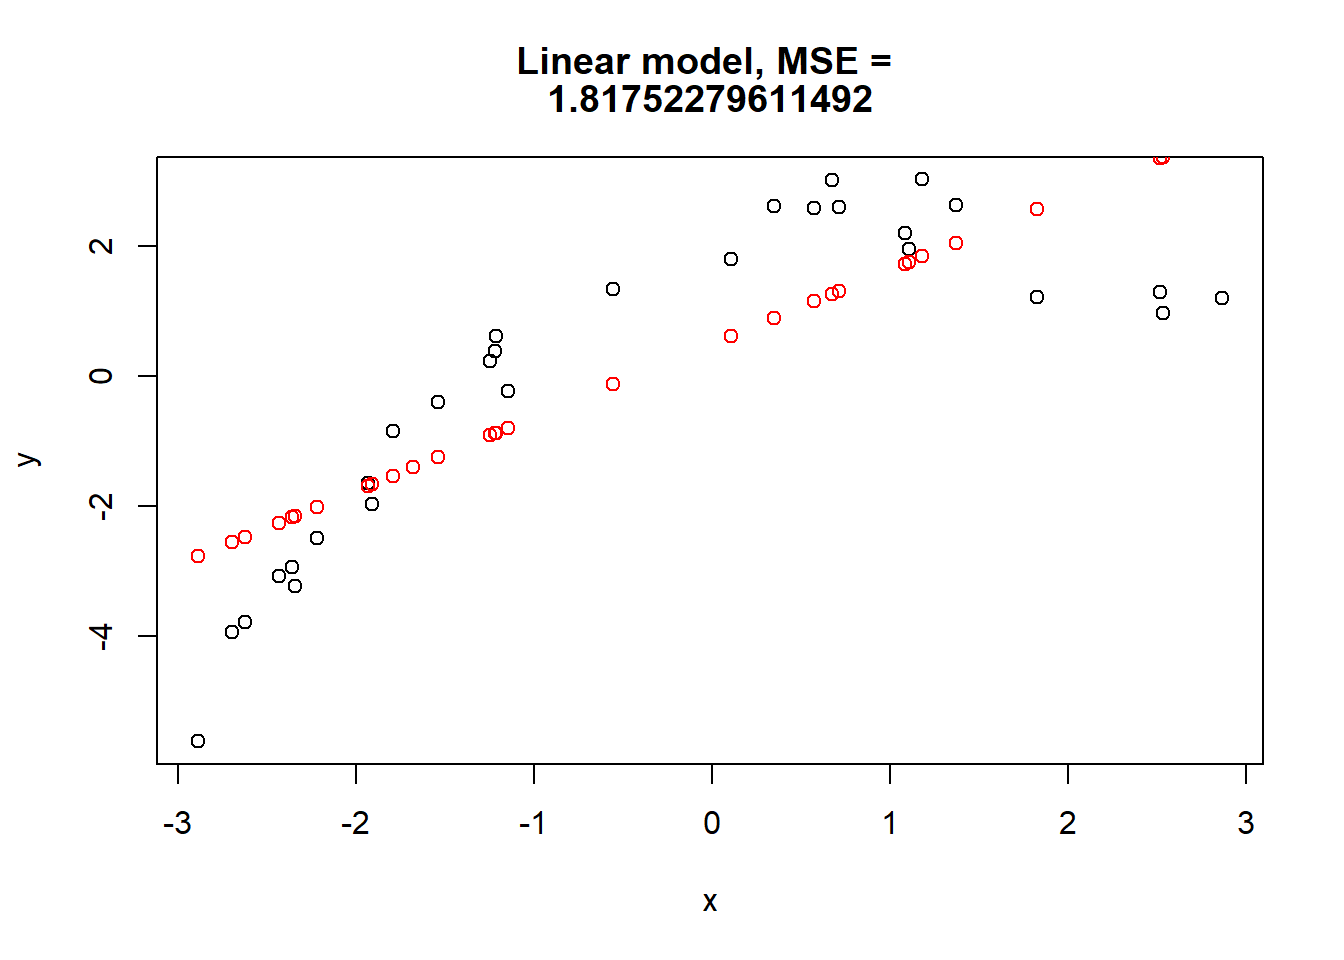
\includegraphics{Week2_files/figure-latex/unnamed-chunk-6-1.pdf}

\begin{Shaded}
\begin{Highlighting}[]
\KeywordTok{persp}\NormalTok{(f1, }\DataTypeTok{theta=}\DecValTok{45}\NormalTok{, }\DataTypeTok{phi=}\DecValTok{35}\NormalTok{)}
\end{Highlighting}
\end{Shaded}

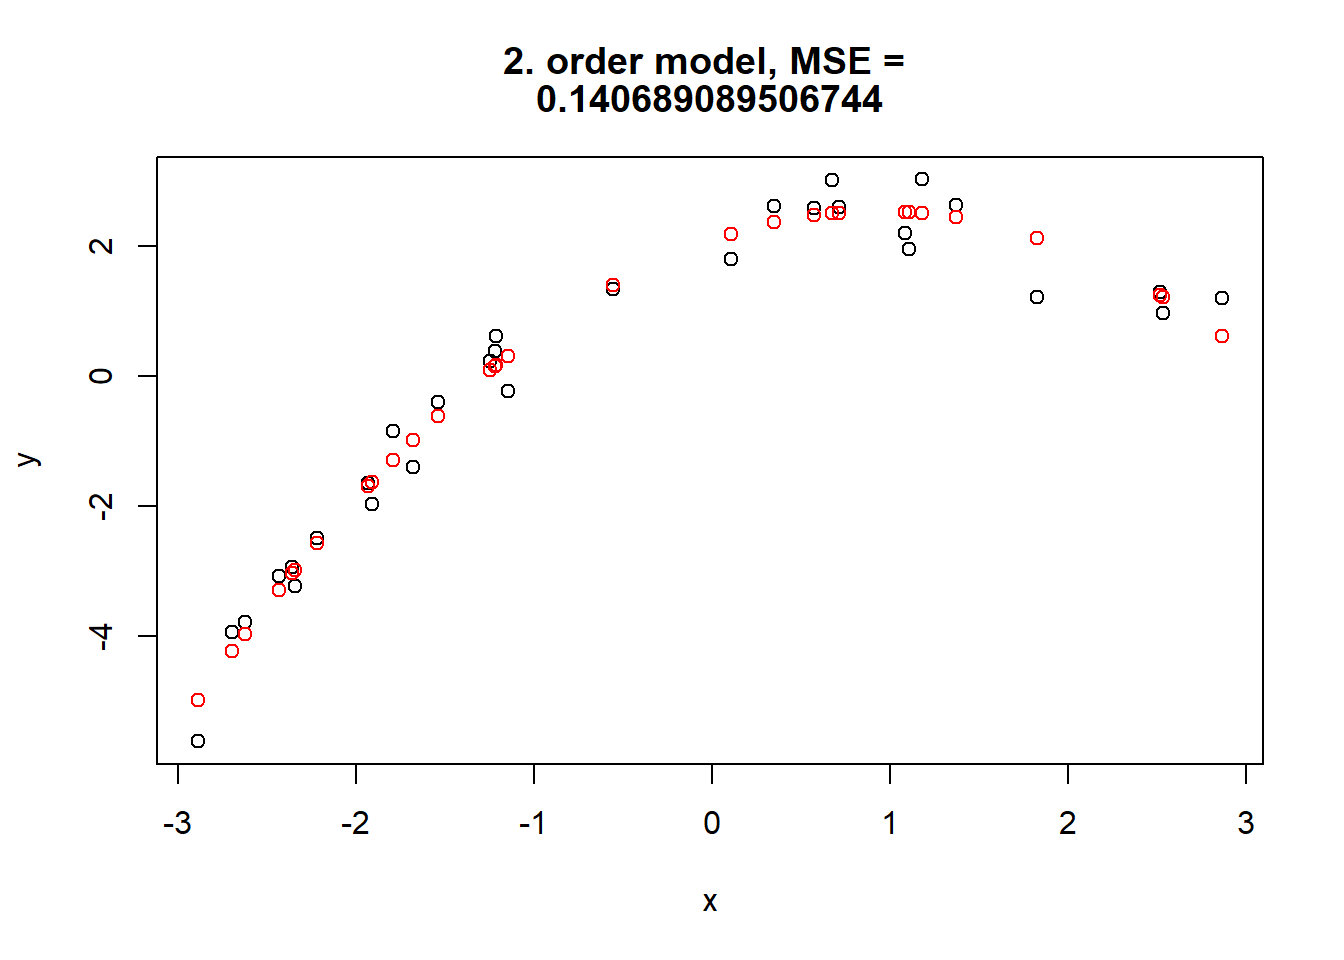
\includegraphics{Week2_files/figure-latex/unnamed-chunk-7-1.pdf} (d) (3
points) Here comes the challenge. (But don't give up: you're almost
there! You should really consider working together with other students
to solve hard exercises like this one.) Denote the mean vector in items
(a)--(c) by µ1 = (0, 0), and let µ2 = (2, 1). Compute the density at the
same set of grid points as in item (c) under distribution N (µ2, Σ),
i.e., with a different mean but the same covariance matrix. Denote the
two densities by fi(x) = N (x ; µi , Σ), i ∈ \{ 1, 2 \}. Calculate the
ratio p(Y = 1 \textbar{} x) = f1(x)π1 f1(x)π1 + f2(x)π2 , with π1 = π2 =
1/2. We will later learn that this is in fact a linear discriminant. Or
to be more precise, this is the posterior probability of class Y = 1
given x. Visualize the decision boundary using, e.g., contour. As the
name suggests, you should get a linear boundary. If you like, you can
now try how well your classifier works by drawing data from either class
and evaluating the above formula. What happens if you use different
covariance matrices Σ1 and Σ2?

\begin{Shaded}
\begin{Highlighting}[]
\CommentTok{#create grid }
\NormalTok{xgrid <-}\StringTok{ }\FloatTok{.25}\OperatorTok{*}\NormalTok{(}\OperatorTok{-}\DecValTok{20}\OperatorTok{:}\DecValTok{20}\NormalTok{)}
\NormalTok{ygrid <-}\StringTok{ }\FloatTok{.25}\OperatorTok{*}\NormalTok{(}\OperatorTok{-}\DecValTok{20}\OperatorTok{:}\DecValTok{20}\NormalTok{)}
\NormalTok{grid <-}\StringTok{ }\KeywordTok{expand.grid}\NormalTok{(xgrid, ygrid)}

\CommentTok{#create the joint distribution on the grid}
\NormalTok{corr =}\StringTok{ }\KeywordTok{c}\NormalTok{(}\FloatTok{2.0}\NormalTok{, }\FloatTok{-0.75}\OperatorTok{*}\KeywordTok{sqrt}\NormalTok{(}\DecValTok{6}\NormalTok{), }\FloatTok{-0.75}\OperatorTok{*}\KeywordTok{sqrt}\NormalTok{(}\DecValTok{6}\NormalTok{), }\FloatTok{3.0}\NormalTok{)}
\NormalTok{sigma <-}\StringTok{ }\KeywordTok{matrix}\NormalTok{(corr,}\DataTypeTok{nrow=}\DecValTok{2}\NormalTok{, }\DataTypeTok{ncol=}\DecValTok{2}\NormalTok{)}
\NormalTok{my1 =}\StringTok{ }\KeywordTok{c}\NormalTok{(}\DecValTok{0}\NormalTok{,}\DecValTok{0}\NormalTok{)}
\CommentTok{#use function dmvnorm of library mvtnorm}
\KeywordTok{library}\NormalTok{(mvtnorm)}
\NormalTok{density1 <-}\StringTok{ }\KeywordTok{dmvnorm}\NormalTok{(grid, }\DataTypeTok{mean=}\NormalTok{my1, }\DataTypeTok{sigma =}\NormalTok{ sigma)}
\NormalTok{density1 <-}\StringTok{ }\KeywordTok{matrix}\NormalTok{(density1, }\DataTypeTok{nrow=}\DecValTok{41}\NormalTok{, }\DataTypeTok{ncol=}\DecValTok{41}\NormalTok{)}

\CommentTok{#draw the distribution}
\KeywordTok{par}\NormalTok{(}\DataTypeTok{mfrow=}\KeywordTok{c}\NormalTok{(}\DecValTok{2}\NormalTok{,}\DecValTok{2}\NormalTok{))}
\KeywordTok{contour}\NormalTok{(xgrid, ygrid, density1)}
\KeywordTok{image}\NormalTok{(xgrid, ygrid, density1)}
\KeywordTok{persp}\NormalTok{(xgrid, ygrid, density1)}
\end{Highlighting}
\end{Shaded}

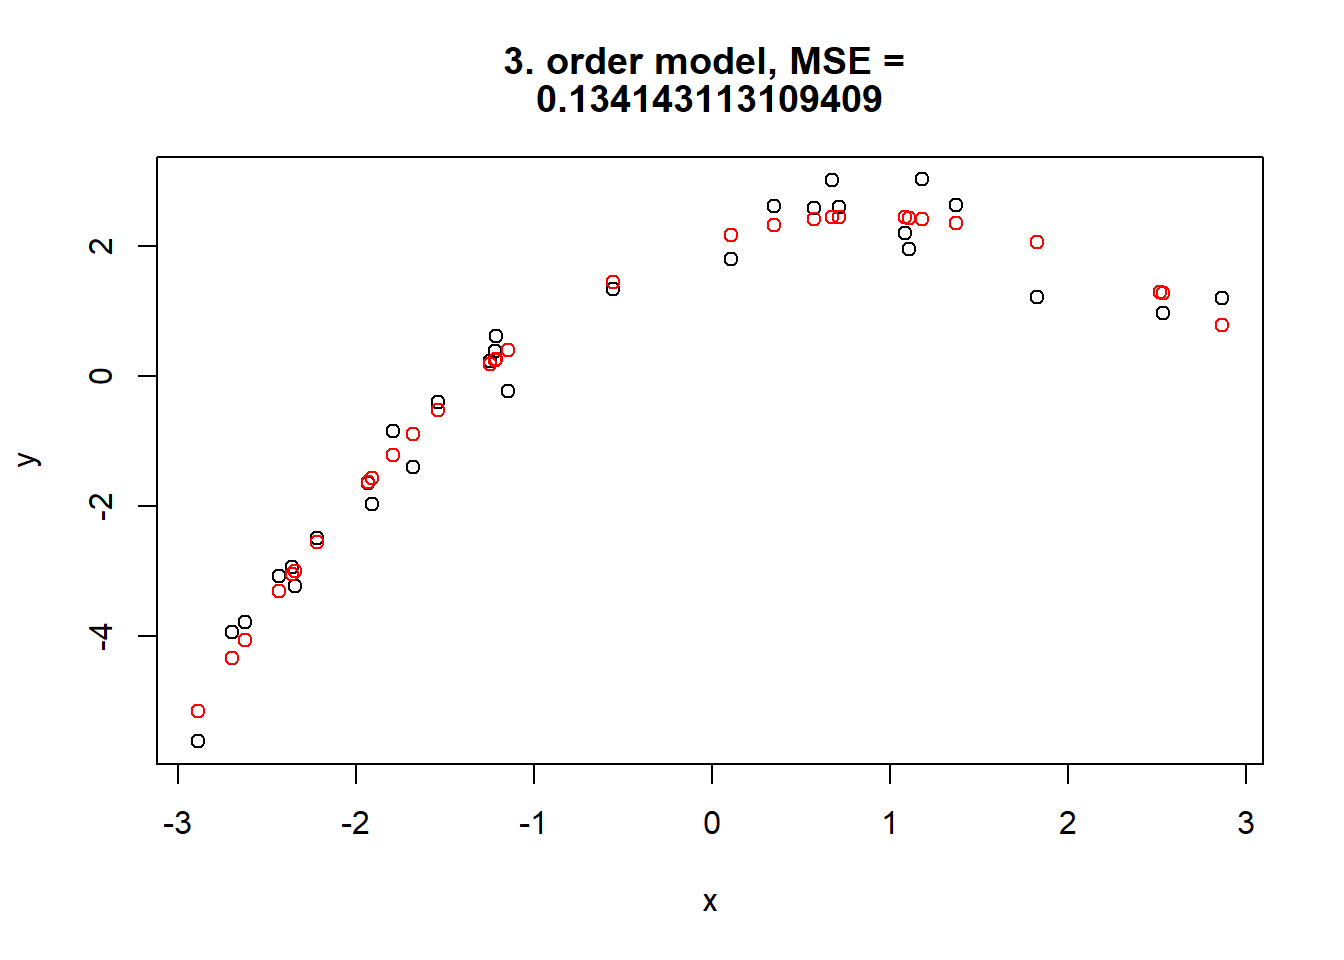
\includegraphics{Week2_files/figure-latex/unnamed-chunk-8-1.pdf}

\begin{Shaded}
\begin{Highlighting}[]
\CommentTok{#Distribution 2:}
\CommentTok{#create grid }
\NormalTok{xgrid <-}\StringTok{ }\FloatTok{.25}\OperatorTok{*}\NormalTok{(}\OperatorTok{-}\DecValTok{20}\OperatorTok{:}\DecValTok{20}\NormalTok{)}
\NormalTok{ygrid <-}\StringTok{ }\FloatTok{.25}\OperatorTok{*}\NormalTok{(}\OperatorTok{-}\DecValTok{20}\OperatorTok{:}\DecValTok{20}\NormalTok{)}
\NormalTok{grid <-}\StringTok{ }\KeywordTok{expand.grid}\NormalTok{(xgrid, ygrid)}

\CommentTok{#create the joint distribution on the grid}
\NormalTok{corr =}\StringTok{ }\KeywordTok{c}\NormalTok{(}\FloatTok{2.0}\NormalTok{, }\FloatTok{-0.75}\OperatorTok{*}\KeywordTok{sqrt}\NormalTok{(}\DecValTok{6}\NormalTok{), }\FloatTok{-0.75}\OperatorTok{*}\KeywordTok{sqrt}\NormalTok{(}\DecValTok{6}\NormalTok{), }\FloatTok{3.0}\NormalTok{)}
\NormalTok{sigma <-}\StringTok{ }\KeywordTok{matrix}\NormalTok{(corr,}\DataTypeTok{nrow=}\DecValTok{2}\NormalTok{, }\DataTypeTok{ncol=}\DecValTok{2}\NormalTok{)}
\NormalTok{my2 =}\StringTok{ }\KeywordTok{c}\NormalTok{(}\DecValTok{2}\NormalTok{,}\DecValTok{1}\NormalTok{)}
\CommentTok{#use function dmvnorm of library mvtnorm}
\CommentTok{#library(mvtnorm)}
\NormalTok{density2 <-}\StringTok{ }\KeywordTok{dmvnorm}\NormalTok{(grid, }\DataTypeTok{mean=}\NormalTok{my2, }\DataTypeTok{sigma =}\NormalTok{ sigma)}
\NormalTok{density2 <-}\StringTok{ }\KeywordTok{matrix}\NormalTok{(density2, }\DataTypeTok{nrow=}\DecValTok{41}\NormalTok{, }\DataTypeTok{ncol=}\DecValTok{41}\NormalTok{)}

\CommentTok{#draw the distribution}
\KeywordTok{par}\NormalTok{(}\DataTypeTok{mfrow=}\KeywordTok{c}\NormalTok{(}\DecValTok{1}\NormalTok{,}\DecValTok{2}\NormalTok{))}
\KeywordTok{contour}\NormalTok{(xgrid, ygrid, density1)}
\KeywordTok{contour}\NormalTok{(xgrid, ygrid, density2)}
\end{Highlighting}
\end{Shaded}

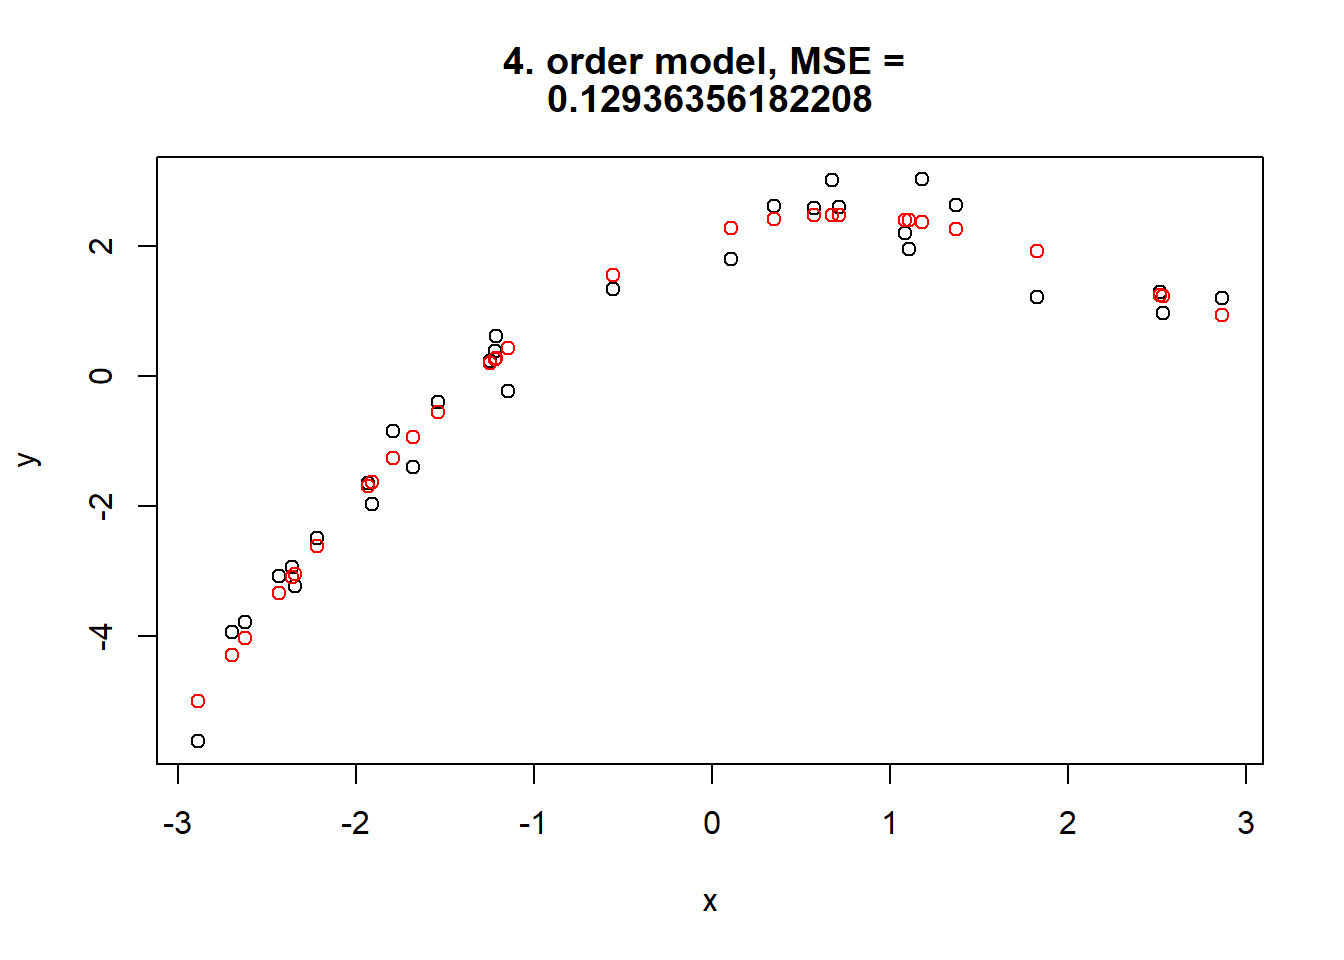
\includegraphics{Week2_files/figure-latex/unnamed-chunk-9-1.pdf}

\begin{Shaded}
\begin{Highlighting}[]
\KeywordTok{par}\NormalTok{(}\DataTypeTok{mfrow=}\KeywordTok{c}\NormalTok{(}\DecValTok{1}\NormalTok{,}\DecValTok{2}\NormalTok{))}
\KeywordTok{persp}\NormalTok{(xgrid, ygrid, density1)}
\KeywordTok{persp}\NormalTok{(xgrid, ygrid, density2)}
\end{Highlighting}
\end{Shaded}

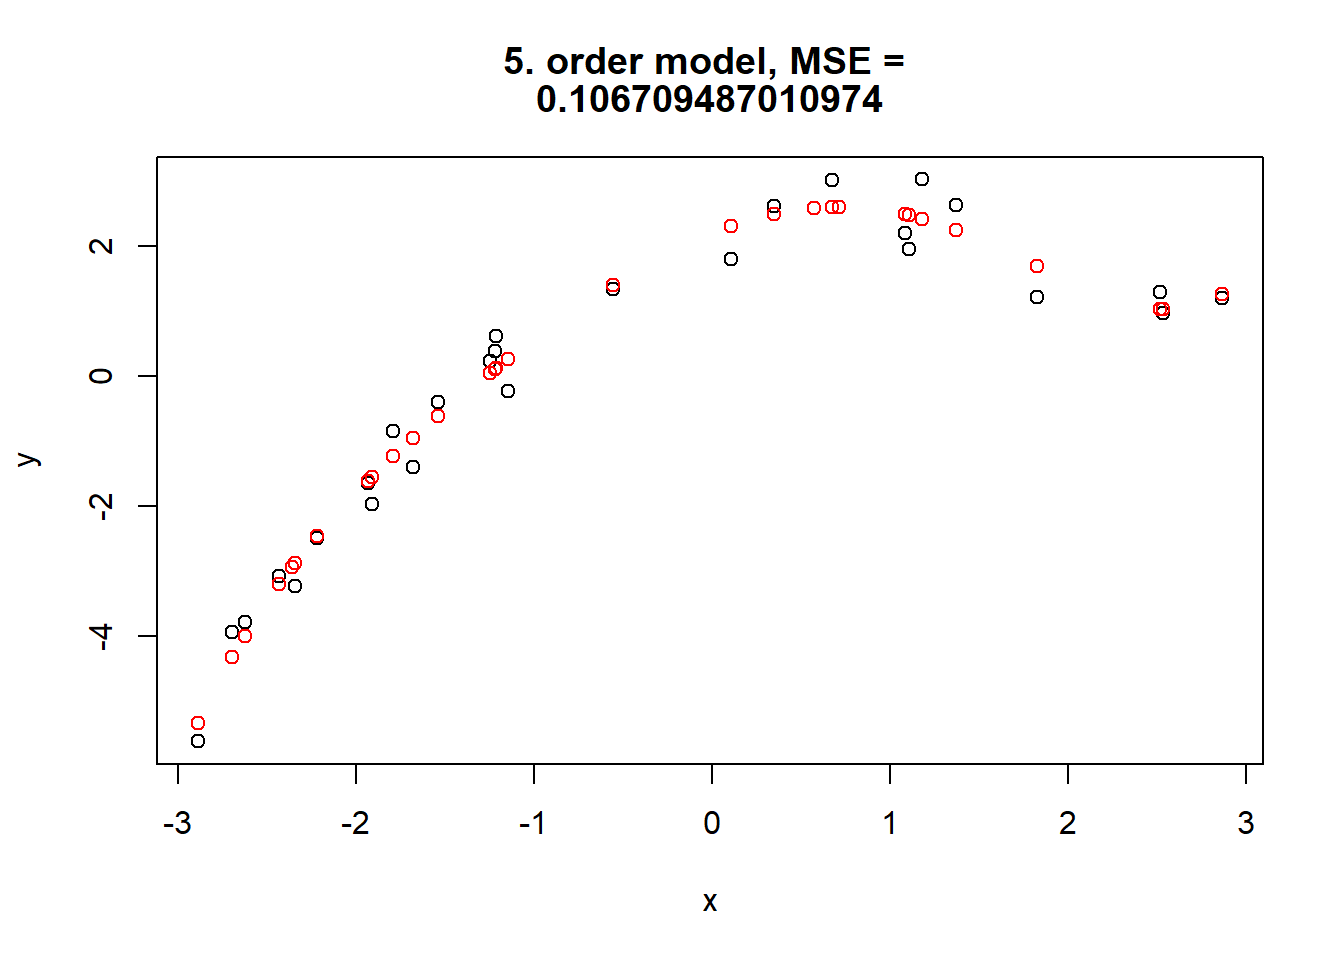
\includegraphics{Week2_files/figure-latex/unnamed-chunk-10-1.pdf}

\begin{Shaded}
\begin{Highlighting}[]
\KeywordTok{par}\NormalTok{(}\DataTypeTok{mfrow=}\KeywordTok{c}\NormalTok{(}\DecValTok{1}\NormalTok{,}\DecValTok{2}\NormalTok{))}
\KeywordTok{image}\NormalTok{(xgrid, ygrid, density1)}
\KeywordTok{image}\NormalTok{(xgrid, ygrid, density2)}
\end{Highlighting}
\end{Shaded}

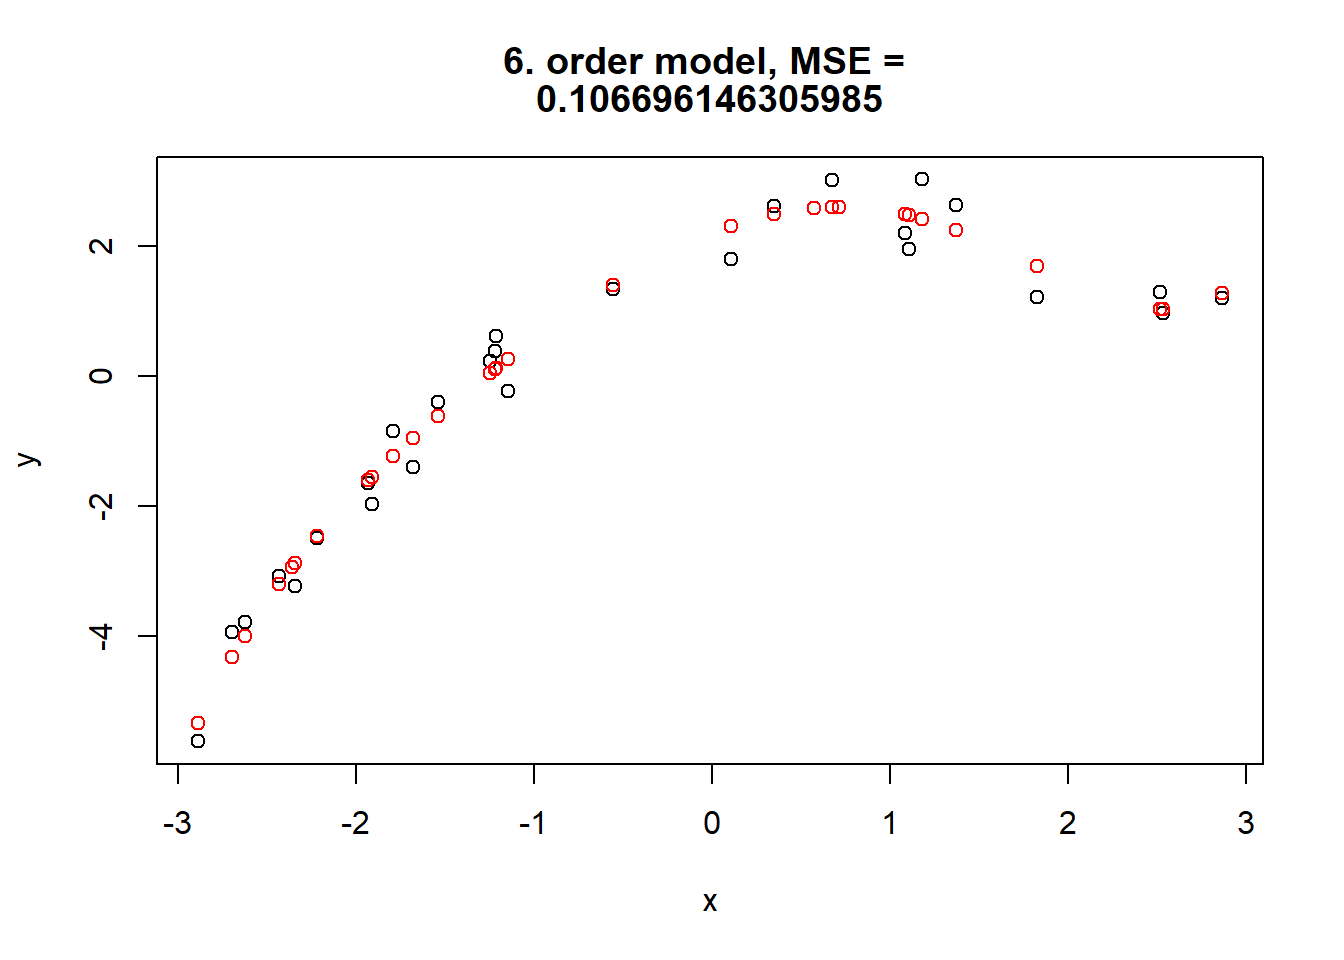
\includegraphics{Week2_files/figure-latex/unnamed-chunk-11-1.pdf}

\begin{Shaded}
\begin{Highlighting}[]
\NormalTok{f1 <-}\StringTok{ }\NormalTok{density1}
\NormalTok{f2 <-}\StringTok{ }\NormalTok{density2}

\NormalTok{lindist =}\StringTok{ }\FloatTok{0.5}\OperatorTok{*}\NormalTok{f1}\OperatorTok{/}\NormalTok{(}\FloatTok{0.5}\OperatorTok{*}\NormalTok{f1 }\OperatorTok{+}\StringTok{ }\FloatTok{0.5}\OperatorTok{*}\NormalTok{f2)}
\KeywordTok{image}\NormalTok{(xgrid, ygrid, lindist)}
\end{Highlighting}
\end{Shaded}

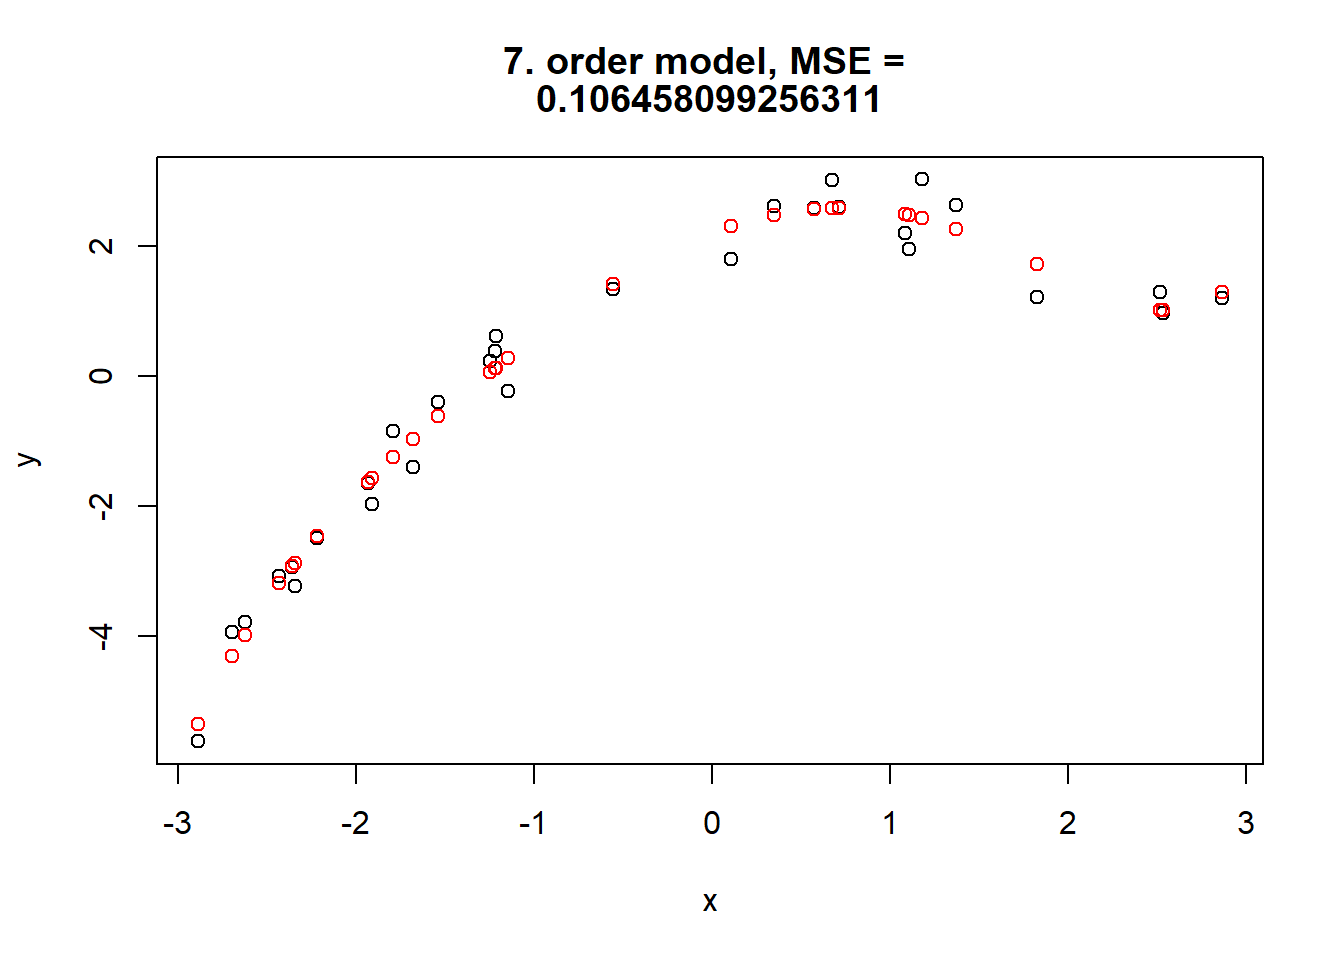
\includegraphics{Week2_files/figure-latex/unnamed-chunk-12-1.pdf}

Experiment with different covariance matrix for the second density, e.g.
\[
\sum_{2}=\begin{bmatrix}
    Cov(X_1, X_1) & Cov(X_1, X_2)\\
    Cov(X_2, X_1) & Cov(X_2, X_2)\\
\end{bmatrix}
=\begin{bmatrix}
    3.0 & \sqrt{6}\\
    \sqrt{6} & 2.5\\
\end{bmatrix}
\]

\begin{Shaded}
\begin{Highlighting}[]
\CommentTok{#Distribution 3:}
\CommentTok{#create grid }
\CommentTok{#create the joint distribution on the grid}
\NormalTok{corr =}\StringTok{ }\KeywordTok{c}\NormalTok{(}\FloatTok{4.0}\NormalTok{, }\KeywordTok{sqrt}\NormalTok{(}\DecValTok{6}\NormalTok{), }\KeywordTok{sqrt}\NormalTok{(}\DecValTok{6}\NormalTok{), }\FloatTok{5.5}\NormalTok{)}
\NormalTok{sigma3 <-}\StringTok{ }\KeywordTok{matrix}\NormalTok{(corr,}\DataTypeTok{nrow=}\DecValTok{2}\NormalTok{, }\DataTypeTok{ncol=}\DecValTok{2}\NormalTok{)}
\NormalTok{my3 =}\StringTok{ }\KeywordTok{c}\NormalTok{(}\DecValTok{2}\NormalTok{,}\DecValTok{1}\NormalTok{)}
\CommentTok{#use function dmvnorm of library mvtnorm}
\CommentTok{#library(mvtnorm)}
\NormalTok{density3 <-}\StringTok{ }\KeywordTok{dmvnorm}\NormalTok{(grid, }\DataTypeTok{mean=}\NormalTok{my3, }\DataTypeTok{sigma =}\NormalTok{ sigma3)}
\NormalTok{density3 <-}\StringTok{ }\KeywordTok{matrix}\NormalTok{(density3, }\DataTypeTok{nrow=}\DecValTok{41}\NormalTok{, }\DataTypeTok{ncol=}\DecValTok{41}\NormalTok{)}

\NormalTok{f3 <-}\StringTok{ }\NormalTok{density3}

\NormalTok{lindist =}\StringTok{ }\FloatTok{0.5}\OperatorTok{*}\NormalTok{f1}\OperatorTok{/}\NormalTok{(}\FloatTok{0.5}\OperatorTok{*}\NormalTok{f1 }\OperatorTok{+}\StringTok{ }\FloatTok{0.5}\OperatorTok{*}\NormalTok{f3)}
\KeywordTok{image}\NormalTok{(xgrid, ygrid, lindist)}
\end{Highlighting}
\end{Shaded}

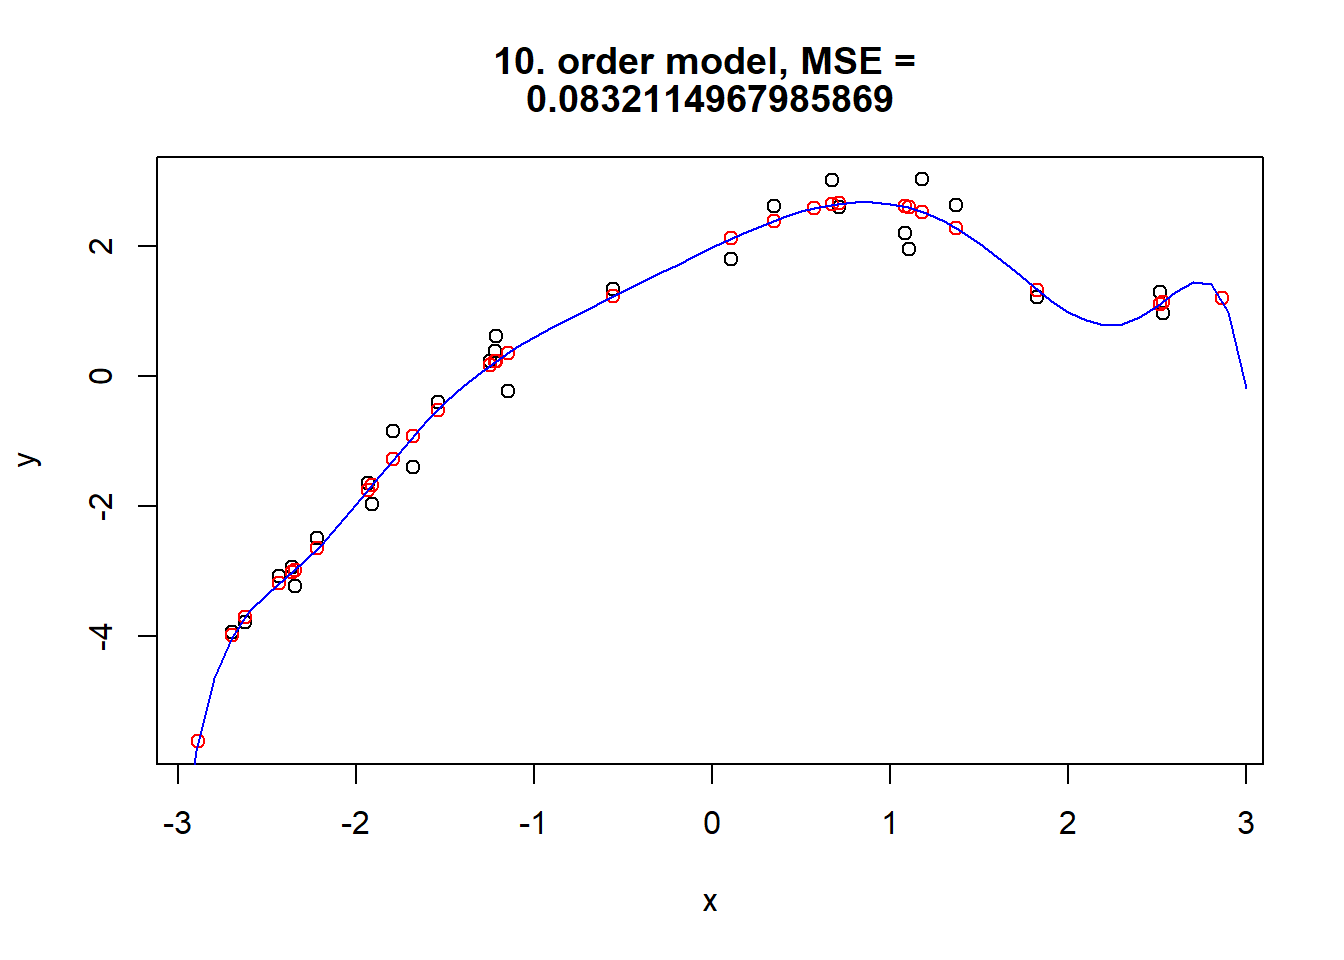
\includegraphics{Week2_files/figure-latex/unnamed-chunk-13-1.pdf}

If you like, you can now try how well your classifier works by drawing
data from either class and evaluating the above formula.

\begin{Shaded}
\begin{Highlighting}[]
\NormalTok{LinDist <-}\StringTok{ }\ControlFlowTok{function}\NormalTok{(point, density1, density2,grid)}
\NormalTok{\{}
\NormalTok{  px =}\StringTok{ }\KeywordTok{which.min}\NormalTok{(}\KeywordTok{abs}\NormalTok{(point[}\DecValTok{1}\NormalTok{] }\OperatorTok{-}\StringTok{ }\NormalTok{grid)) }
\NormalTok{  py =}\StringTok{ }\KeywordTok{which.min}\NormalTok{(}\KeywordTok{abs}\NormalTok{(point[}\DecValTok{2}\NormalTok{] }\OperatorTok{-}\StringTok{ }\NormalTok{grid))}
    
\NormalTok{  f1 <-}\StringTok{ }\NormalTok{density1[px,py]}
\NormalTok{  f2 <-}\StringTok{ }\NormalTok{density2[px,py]}
  \KeywordTok{return}\NormalTok{ (}\FloatTok{0.5}\OperatorTok{*}\NormalTok{f1}\OperatorTok{/}\NormalTok{(}\FloatTok{0.5}\OperatorTok{*}\NormalTok{f1 }\OperatorTok{+}\StringTok{ }\FloatTok{0.5}\OperatorTok{*}\NormalTok{f2))}
\NormalTok{\}}
\end{Highlighting}
\end{Shaded}

\begin{Shaded}
\begin{Highlighting}[]
\CommentTok{#draw two samples from the two distributions}
\NormalTok{c1 <-}\StringTok{ }\KeywordTok{c}\NormalTok{()}
\NormalTok{c2 <-}\StringTok{ }\KeywordTok{c}\NormalTok{()}
\ControlFlowTok{for}\NormalTok{(i }\ControlFlowTok{in} \DecValTok{1}\OperatorTok{:}\DecValTok{100}\NormalTok{)}
\NormalTok{\{}
\NormalTok{  s2 <-}\StringTok{ }\KeywordTok{rmvnorm}\NormalTok{(}\DecValTok{1}\NormalTok{, }\DataTypeTok{mean=}\NormalTok{my2, }\DataTypeTok{sigma =}\NormalTok{ sigma)}
\NormalTok{  c1<-}\StringTok{ }\KeywordTok{c}\NormalTok{(c1, }\KeywordTok{LinDist}\NormalTok{(s2, density1, density2,xgrid))}
\NormalTok{  c2<-}\StringTok{ }\KeywordTok{c}\NormalTok{(c2, }\KeywordTok{LinDist}\NormalTok{(s2, density2, density1,xgrid))}
\NormalTok{\}}
\KeywordTok{sum}\NormalTok{(c1 }\OperatorTok{<}\StringTok{ }\FloatTok{0.5}\NormalTok{)}\OperatorTok{/}\DecValTok{100}
\end{Highlighting}
\end{Shaded}

\begin{verbatim}
## [1] 0.98
\end{verbatim}


\end{document}
